\documentclass[12pt]{article}

% import packages
\usepackage[utf8]{inputenc}
\usepackage{float}
\usepackage{subfloat}
\usepackage{subfig}
\usepackage{amsmath}
\usepackage[toc,page]{appendix}
\usepackage{caption}
\usepackage{graphicx}
\usepackage{hyperref}
\usepackage[left=1in,top=0.75in,right=1in,bottom=0.75in]{geometry}

\graphicspath{ {./images} }
% hyperref setup
\hypersetup{
	colorlinks=true,
	linkcolor=blue,
	filecolor=blue,      
	urlcolor=blue,
	citecolor=blue,
	pdftitle={Investigation into vehicle motion measurement techniques},
	pdfpagemode=FullScreen,
}
% titlepage	
\title{\textbf{Investigation into vehicle motion measurement techniques}}
\author{Callum Stephenson, css47, GRP173, Car4, Trinity}
\date{}

\begin{document}
    \begin{titlepage}
        \maketitle
        \thispagestyle{empty}
        \vspace{13cm}
        \textbf{Department of Engineering, University of Cambridge}
    \end{titlepage}
    \tableofcontents
    \newpage
    \section{Introduction}
    The aim of this report is to determine which techniques for analysing vehicle motion are most accurate, as well as 
    understanding how they are able to track a specific quantity about the vehicle. 
    
    Within this report, a model 1:18 488 GTB equipped with sensors will be used in order to investigate the performance of
    different sensors on the car. Being able to track the motion of a vehicle accurately is useful when trying to determine path,
    or to change certain values within the engine to increase effiency or maintain a set speed. One aspect to accuracy is the calibration of
    a measurement device between digital and real world steps. This is done on the model vehicle within this experiment similarly to
    how one might calibrate e-steps on a 3D printing machine by counting the movement in the axis comparative to rotation in the stepper motor.
    \newpage
    \section{Figures, answers to questions \& bullet points}
    \subsection{Initial sensor readings}
    \begin{figure}[H]
        \captionsetup{labelfont=bf}
        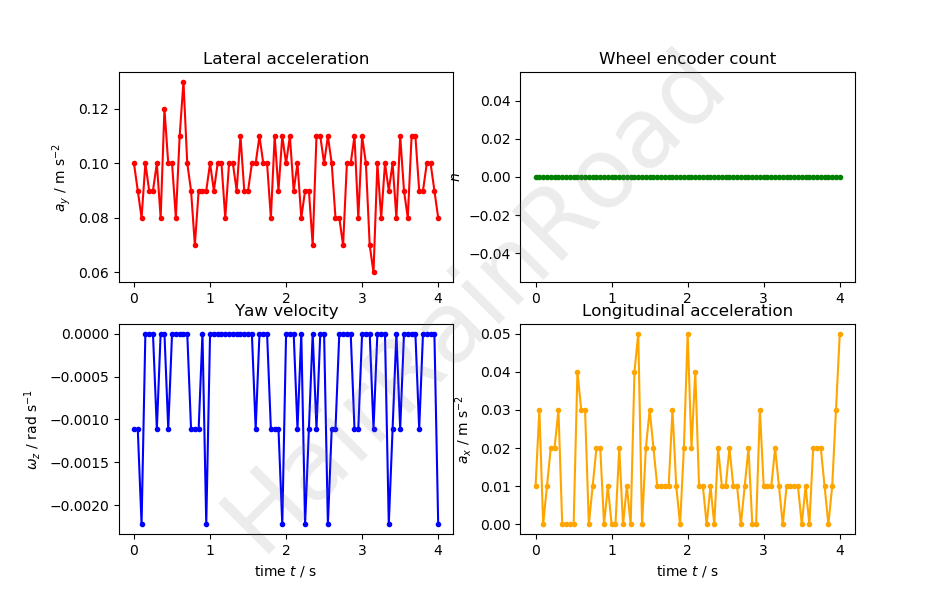
\includegraphics[width=40pc]{fig1png.png}
        \caption{Initial readings from sensors with no motion of the vehicle}\label{figure1}
    \end{figure}
    \begin{itemize}
        \item The sample rate is 20 Hz, this can be confirmed by counting the amount of data points per second, gives a result of 20 per 
        second which is consistent with one every 50 ms.
        \item Quantization step size for each of the four signals. Lateral acceleration: 0.02 ms$^{-2}$, Yaw velocity: 0.0012 ms$^{-1}$,
        Longitudinal acceleration: 0.01 ms$^{-2}$, Rotary encoder 1 (step).
        \item Mean value of each signal. Lateral acceleration: 0.09 ms$^{-2}$, Yaw velocity: -0.0012 ms$^{-1}$,
        Longitudinal acceleration: 0.01 ms$^{-2}$, Rotary encoder 0 (step). It is as you would expect, negligible values when not moving.
        \item Approximate peak-to-peak of each signal. Lateral acceleration: 0.06 ms$^{-2}$, Yaw velocity: 0.0024 ms$^{-1}$,
        Longitudinal acceleration: 0.05 ms$^{-2}$, Rotary encoder 0 (step). Peak to peak is also as expected, very small and negligible comparative to measurements later.
        \item Calibration is required in order to have correct output on the sensors. You can do this by moving a known distance, 
        and calculating the amount of virtual steps that are moved. 
    \end{itemize}
    \newpage
    \subsection{Calibration of rotary encoder}
    \begin{figure}[H]
        \captionsetup{labelfont=bf}
        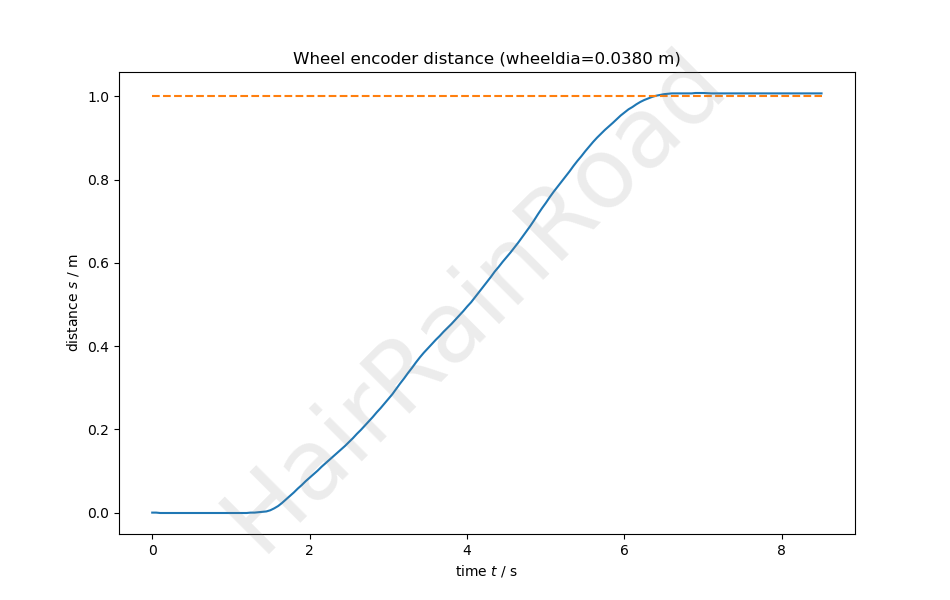
\includegraphics[width=40pc]{fig2png.png}
        \caption{Rotary wheel readings converted to distance(m) per time (s)}\label{figure2}
    \end{figure}
    \begin{itemize}
    \item Before calibration, the measured distance by rotary encoder was not the same as the actual distance on the tapemeasure.
    \item This means that the rotary encoder e-steps are wrong, this requires calibration. The calculation to get the distance per rotation
    is to do with the wheel diameter as the only other variable beside distance moved. (Assuming no slip.)
    \item We re-measured the wheel diameter. It came out to be around 0.38m, not the original 0.4 inputted into the program.
    \item Using this new measurement for wheel diameter, we repeated the experiment and it can be seen that the distance lined up correctly
    with the actual distance travelled.
    \end{itemize}
    \newpage
    \subsection{Comparing IMU measurements to the wheel encoder}
    \begin{figure}[H]
        \captionsetup{labelfont=bf}
        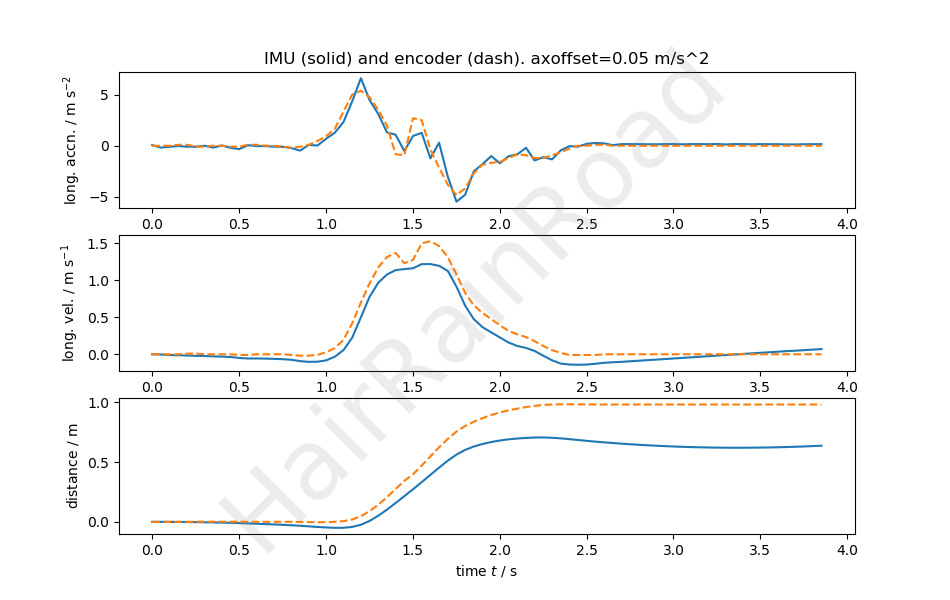
\includegraphics[width=40pc]{fig3png.png}
        \caption{Measurements from both the IMU and rotary wheel encoder compared}\label{figure3}
    \end{figure}
    \begin{itemize}
        \item The data is not as expected, as the velocity dips negative when the car was only ever moved in a straight line.
        \item The velocity and acceleration are close, but the distance has a large disparity between IMU and the rotary encoder.
        \item This could be down to the placement of the IMU and rotary encoder, where the encoder is mesauring the distance
        travelled by the left wheel, and the IMU measures the movement of the centre of mass.
        \item The jitter of the measurements measured in \ref{figure1} may explain why the velocity does not end at 0.
        \item We added an ax offset in order to bring the velocity at the end closer to zero, this brought the graphs closer together
        as can be seen in \ref{figure3}
        \item Our value of axoffset was 0.05. Negative velocity still registered so the axoffset wasn't enough to fix the graphs entirely.
        \item It is possible to compensate for the errors in the inertial sensors, but we have not done so, hence the issues.
    \end{itemize}
    \newpage
    \subsection{Circular motion}
    \subsubsection{Calculation of yaw velocity with IMU}
    \begin{figure}[H]
        \captionsetup{labelfont=bf}
        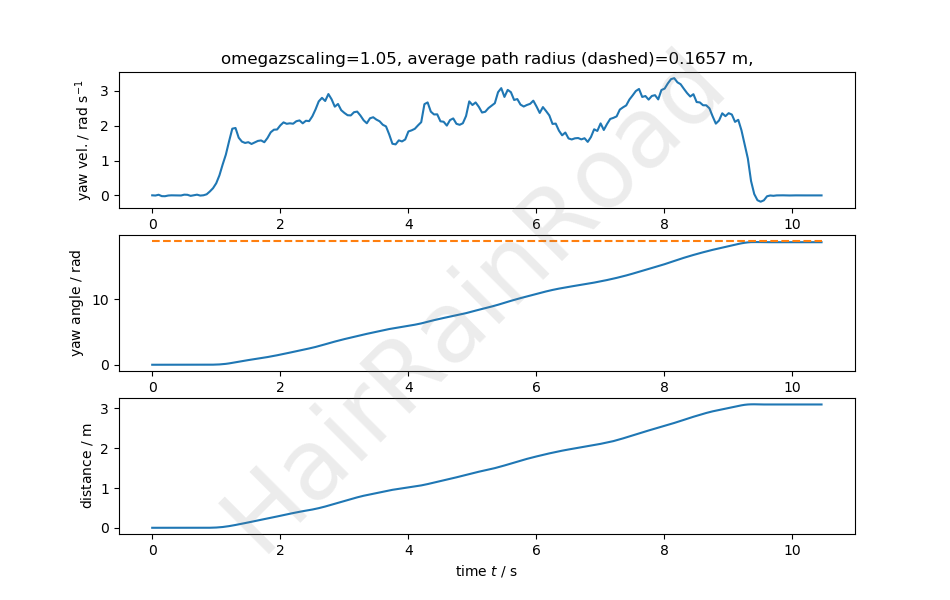
\includegraphics[width=40pc]{fig4png.png}
        \caption{Top: Yaw velocity measured when travelling in three circles, Middle: Yaw angle (dashed = expected end), Bottom: distance from rotary encoder}\label{figure4}
    \end{figure}
    \begin{itemize}
        \item Our average path was measured to be 0.185m. This is similar to the 0.166m calculated by the IMU.
        \item By using the omegazscaling, we were able to get the sensor to register a full circle as we completed one,
        middle figure ends at orange dashed line. 
        \item The middle and bottom graphs are very similar, the bottom graph is data from the calibrated rotary encoder.
        This shows that the yaw velocity is calibrated well, as you would expect a linear relationship between angle rotated through and distance
        \\ (Area of sector = $r \theta$.)
        \item It was hard to measure the radius, and this might be one of the reasons for the slight discrepancy between the measured and actual
        values. 
    \end{itemize}
    \newpage
    \subsubsection{Estimating radius of path using encoder and yaw velocity}
    \begin{figure}[H]
        \captionsetup{labelfont=bf}
        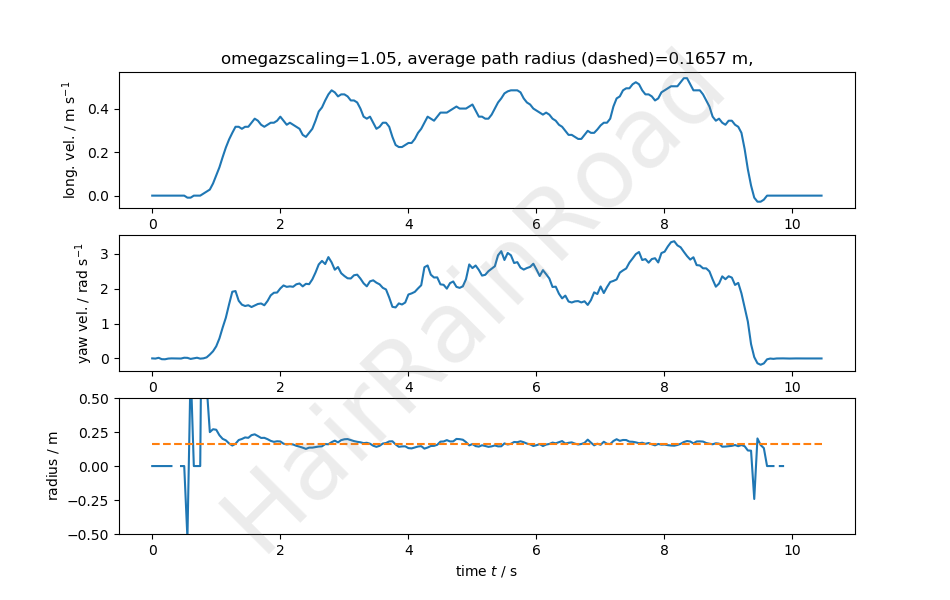
\includegraphics[width=40pc]{fig5png.png}
        \caption{Graph showing the long. vel. , yaw vel. and the division of the two on the bottom.}\label{figure5}
    \end{figure}
    \begin{itemize}
        \item Longitudinal velocity and yaw velocity can be related through the formula $r=\frac{v_x}{\omega_z}$
        \item Now that we have a calibrated longitudinal and yaw velocity, we can use this formula to obtain a radius.
        \item The spikes on the bottom graph are when we stopped and started the car, which would result in two small values dividing giving a huge spike.
        \item However, during the duration of the rotation - the radius was relatively constant and therefore it would be safe to say both sensors
        are relatively well calibrated otherwise there would've been drift.
        \item The top and middle graphs show that the longitudinal and yaw velocity are relatively close.
    \end{itemize}
    \newpage
    \subsubsection{Estimate radius of path using encoder and lateral acceleration}
    \begin{figure}[H]
        \captionsetup{labelfont=bf}
        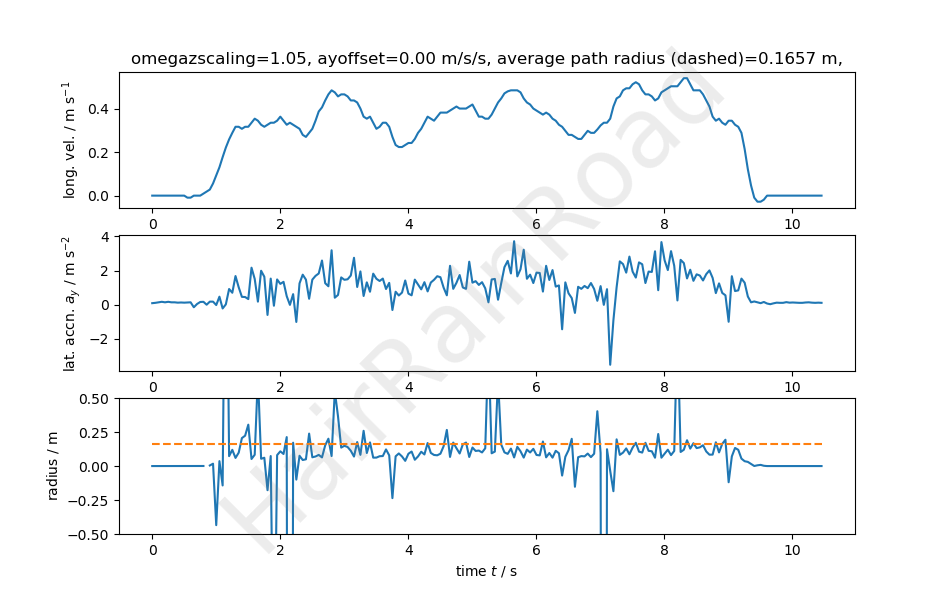
\includegraphics[width=40pc]{fig6png.png}
        \caption{Graphs to show the radius of the circle using longitudinal velocity and lateral acceleration}\label{figure6}
    \end{figure}
    \begin{itemize}
        \item Radius of path can be related to longitudinal velocity and lateral acceleration by $r = \frac{v_x^2}{a_x}$
        \item The radius follows the dashed line less closely than the last graph.
        \item This could be due to the $v_x^2$ term, where errors are squared, resulting in double the uncertainty.
        \item This could explain why the graph is following the dashed line, but with more spikes due to small errors in the $v_x^2$ term.
        \item Another reason for the error is the jittery acceleration graph. There may have been some slippage when moving the car
        which resulted in a jittery accerlation.
    \end{itemize}
    \newpage
    \subsubsection{Estimate path radius using longitudinal acceleration and yaw velocity}
    \begin{figure}[H]
        \captionsetup{labelfont=bf}
        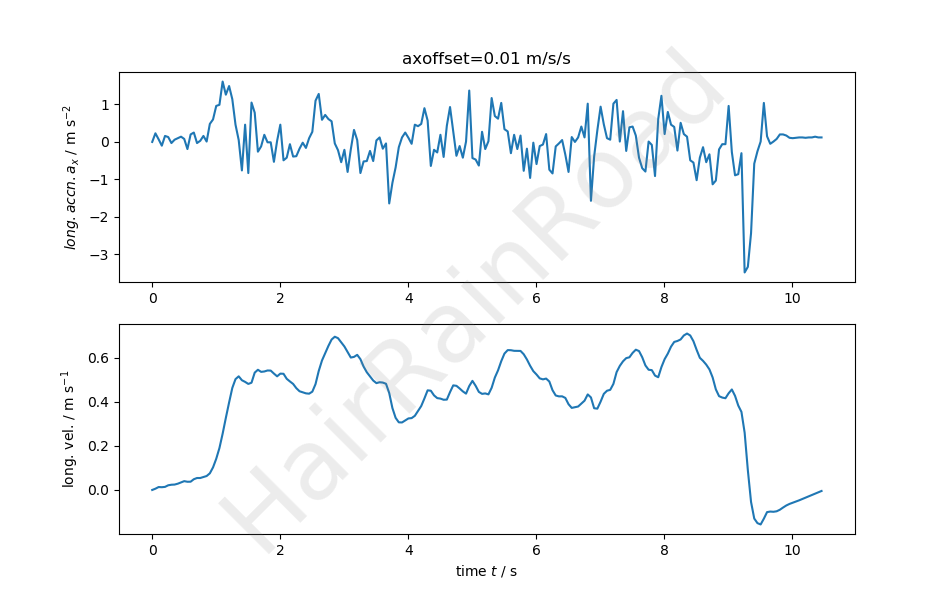
\includegraphics[width=40pc]{fig7png.png}
        \caption{Graphs to show the longitudinal acceleration and yaw velocity}\label{figure7}
    \end{figure}
    \begin{itemize}
        \item $v_x$ is now found by integrating the longitudinal acceleration, still related by $r = \frac{v_x}{\omega_z}$
        \item We need to ensure the offset is zero at the end of the run in order to use this.
        \item We used an axoffset value of 0.01 ms$^{-2}$, it requires a smaller value than the earlier axoffset.
        \item The reason for the smaller value is that it is integrated over, and will become an $x^1$ term. 
        \item Now that we have zero offset, we can do the same graphs as earlier to find the radius of path.
    \end{itemize}
    \newpage
    \begin{figure}[H]
        \captionsetup{labelfont=bf}
        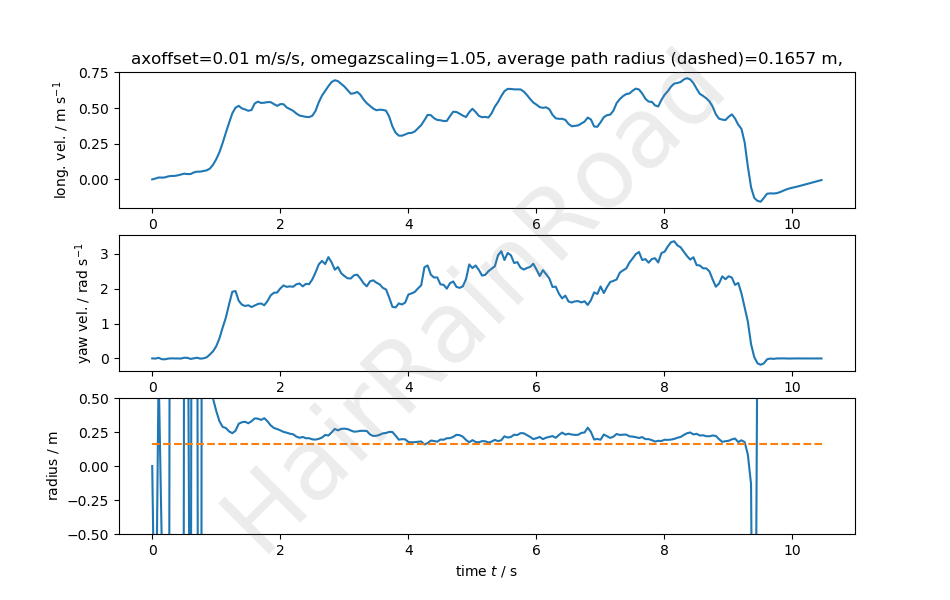
\includegraphics[width=40pc]{fig8png.png}
        \caption{Graphs to show the path radius using longitudinal acceleration and yaw velocity}\label{figure8}
    \end{figure}
    \begin{itemize}
        \item When the yaw velocity is very small, a positive number divided by a very small positive number results in the spikes, 
        as seen earlier.
        \item The radius of path is consistently over the calculated dashed line.
        \item This may be because the mean line is calculated by the IMU, but the rotary encoder is on the left back of the wheel
        so it travels a greater distance overall.
        \item This emphasises the importance of taking position of the sensor within the vehicle into consideration when trying to find a path radius.
    \end{itemize}
    \newpage
    \subsection{Arbitrary path}
    \begin{figure}[H]
        \captionsetup{labelfont=bf}
        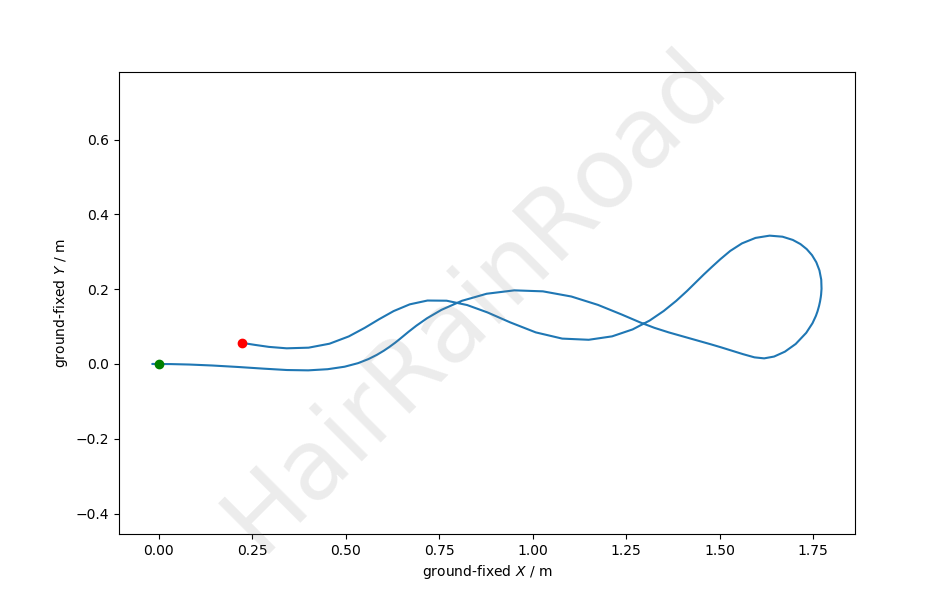
\includegraphics[width=40pc]{fig9png.png}
        \caption{Graph showing our arbitrary path using the calibrated sensors}\label{figure9}
    \end{figure}
    \begin{itemize}
        \item Yes, the path is the same as that which we traced out on the table. We were surprised that the values matched up as well as they did.
        \item Instead of using encoder and yaw velocity, we could have used velocity + sideways velocity but the accuracy of the calibrated
        encoder is far better than the IMU. 
        \item The combination of the yaw velocity and the rotary encoder is similar to an intrinsic coordinate system. 
        \item x displacement = $ \cos \theta$.d, y displacement = $ \sin \theta$.d, where d is the overall distance travelled from rotary encoder and $\theta$
        comes from the yaw angle.
    \end{itemize}
    \newpage
    \section{Conclusion}
    \begin{itemize}
        \item From the figures above it is possible to see that an accurate path can be calculated from combining measurements from the sensors
        in a clever way.
        \item There are many combinations that would successfully give the path, but it is best to pick the sensors with the least susceptibility
        to errors, and hence choosing something like the acceleration would not be the best idea.
        \item As discussed in the bullet points under \ref{figure9}, the careful choice to use yaw angle and rotary encoder distance results 
        in an accurate path which represented the one traced on the table. 
        \item It was important to remember that all sensors need to be calibrated to get the steps:unit, as a sensor such as the rotary sensor
        is not aware of how far it should've travelled per metre, so it is important to have accurate calculations from rotation to distance.
        \item Making sure that inertial sensors have the right offset or multiplier is also key, and using a known reference value like with 
        the rotary encoder is the best way to achieve this.
        \item Knowing set attributes about a vehicle's acceleration is useful if you want to control speed or limit acceleration. The combination
        of speed and power output can also be used to set the gearing in automatic vehicles.
        \item By eliminating square terms, the overall error and uncertainty within the values can be reduced.
        \item When using two or more sensors, it is important to consider the position of the sensors within the vehicle,
        as each can travel a different distance or experience different velocities which could hinder your ability to gather accurate results.
        \item If you were interested in accuracy and were using an IMU, you may be inclined to try to use the inbuilt correction for the effects
        of gravitational fields and sensor offsets and angular velocity sensors. 
        \item Another way to combat error is to use a multitude of sensors and compare the output of many to arrive at an agreed upon value
        between all of the sensors. This would itilise something like a concensus algorithm in order to have a computer decide which value can be taken
        as correct.
    \end{itemize}
\end{document}